\subchapter{Lab5: Extend a recipe}{Add your features to an existing recipe}

During this lab, you will:
\begin{itemize}
  \item Apply patches to an existing recipe
  \item Use a custom configuration file for an existing recipe
  \item Extend a recipe to fit your needs
\end{itemize}

\section{Create a basic appended recipe}

To avoid rewriting recipes when a modification is needed on an already existing
one, BitBake allows to extend recipes and to overwrite, append or prepend
configuration variables values through the so-called BitBake append files.

We will first create a basic BitBake append file, without any change made
to the original recipe, to see how it is integrated into the build. We will then
extend some configuration variables of the original recipe.

Try to create an appended recipe with the help of the online Yocto
Project development documentation. You can find it at
\url{https://www.yoctoproject.org/docs/2.5/dev-manual/dev-manual.html}. We here
aim to extend the \ifdefstring{\labboard}{discovery}{\code{linux-stm32mp}}
{\code{linux-ti-staging}} kernel recipe.

You can see available \code{bbappend} files and the recipe they apply to by
using the \code{bitbake-layers} tool (again!):
\begin{verbatim}
bitbake-layers show-appends
\end{verbatim}

If the BitBake append file you just created is recognized by your Yocto
environment, you should see:
\if\defstring{\labboard}{discovery}
\begin{verbatim}
linux-stm32mp_4.19.bb:
 $HOME/yocto-labs/meta-bootlinlabs/recipes-kernel/linux/linux-stm32mp_4.19.bbappend
\end{verbatim}
\else
\begin{verbatim}
linux-ti-staging_4.14.bb:
  $HOME/yocto-labs/meta-bootlinlabs/recipes-kernel/linux/linux-ti-staging_4.14.bbappend
\end{verbatim}
\fi

\section{Add patches to apply in the recipe}

We want our extended
\ifdefstring{\labboard}{discovery}{\code{linux-stm32mp}}
{\code{linux-ti-staging}} kernel to support the Nunchuk as
a joystick input. We can add this by applying patches during the
\code{do_patch} task. The needed patches are provided with this lab. You can
find them under \code{~/yocto-labs/bootlin-lab-data/nunchuk/linux}. For more
details about how to write the driver handling the Nunchuk, have a look at our
embedded Linux kernel and driver development training course at
\url{https://bootlin.com/training/kernel/}.

Applying a patch is a common task in the daily Yocto process. Many recipes,
appended or not, apply a specific patch on top of a mainline project. It's why
patches do not have to be explicitly applied, if the recipe inherits from the
patch class (directly or not), but only have to be present in the source files
list.

Try adding the patches included in this lab to your BitBake append
file. Do not forget to also add the \code{defconfig} file provided
alongside the patches. This file contains the kernel configuration and
is handled automatically in the \ifdefstring{\labboard}{discovery}{\code{linux-stm32mp}}
{\code{linux-ti-staging}} original recipe.

You can now rebuild the kernel to take the new patches into account:
\begin{verbatim}
bitbake virtual/kernel
\end{verbatim}

\section{Connect the Nunchuk}

Take the Nunchuk device provided by your instructor.

We will connect it to the second I2C port of the CPU (\code{i2c1}),
with pins available on the \code{P9} connector.

Identify the 4 pins of the Nunchuk connector:

\begin{center}
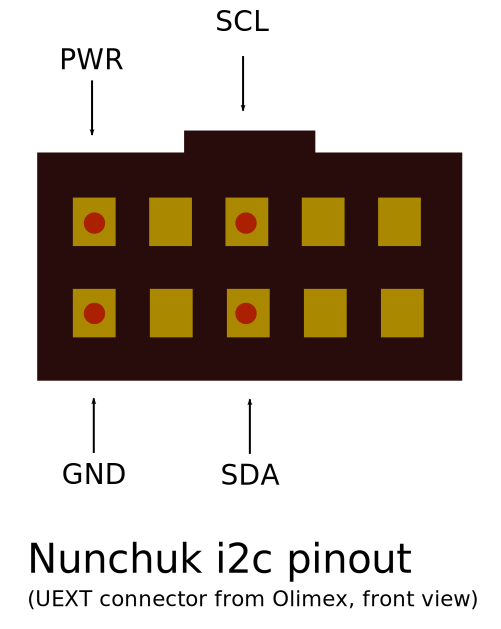
\includegraphics[width=4cm]{common/nunchuk-pinout.pdf}
\end{center}

\ifdefstring{\labboard}{discovery}{
Connect the Nunchuk pins:
\begin{itemize}
\item The \code{GND} pin to CN16 pin 7 (\code{GND})
\item The \code{PWR} pin to CN16 pin 8 (\code{3V3})
\item The \code{DATA} pin to CN13 pin 9 (\code{D14})
\item The \code{CLK} pin to CN13 pin 10 (\code{D15})
\end{itemize}

\begin{center}
  TODO
%\includegraphics[width=12cm]{common/dk2-connect-nunchuk.pdf}
\end{center}
}{
Connect the Nunchuk pins:
\begin{itemize}
\item The \code{GND} pin to P9 pins 1 or 2 (\code{GND})
\item The \code{PWR} pin to P9 pins 3 or 4 (\code{DC_3.3V})
\item The \code{CLK} pin to P9 pin 17 (\code{I2C1_SCL})
\item The \code{DATA} pin to P9 pin 18 (\code{I2C1_SDA})
\end{itemize}

\begin{center}
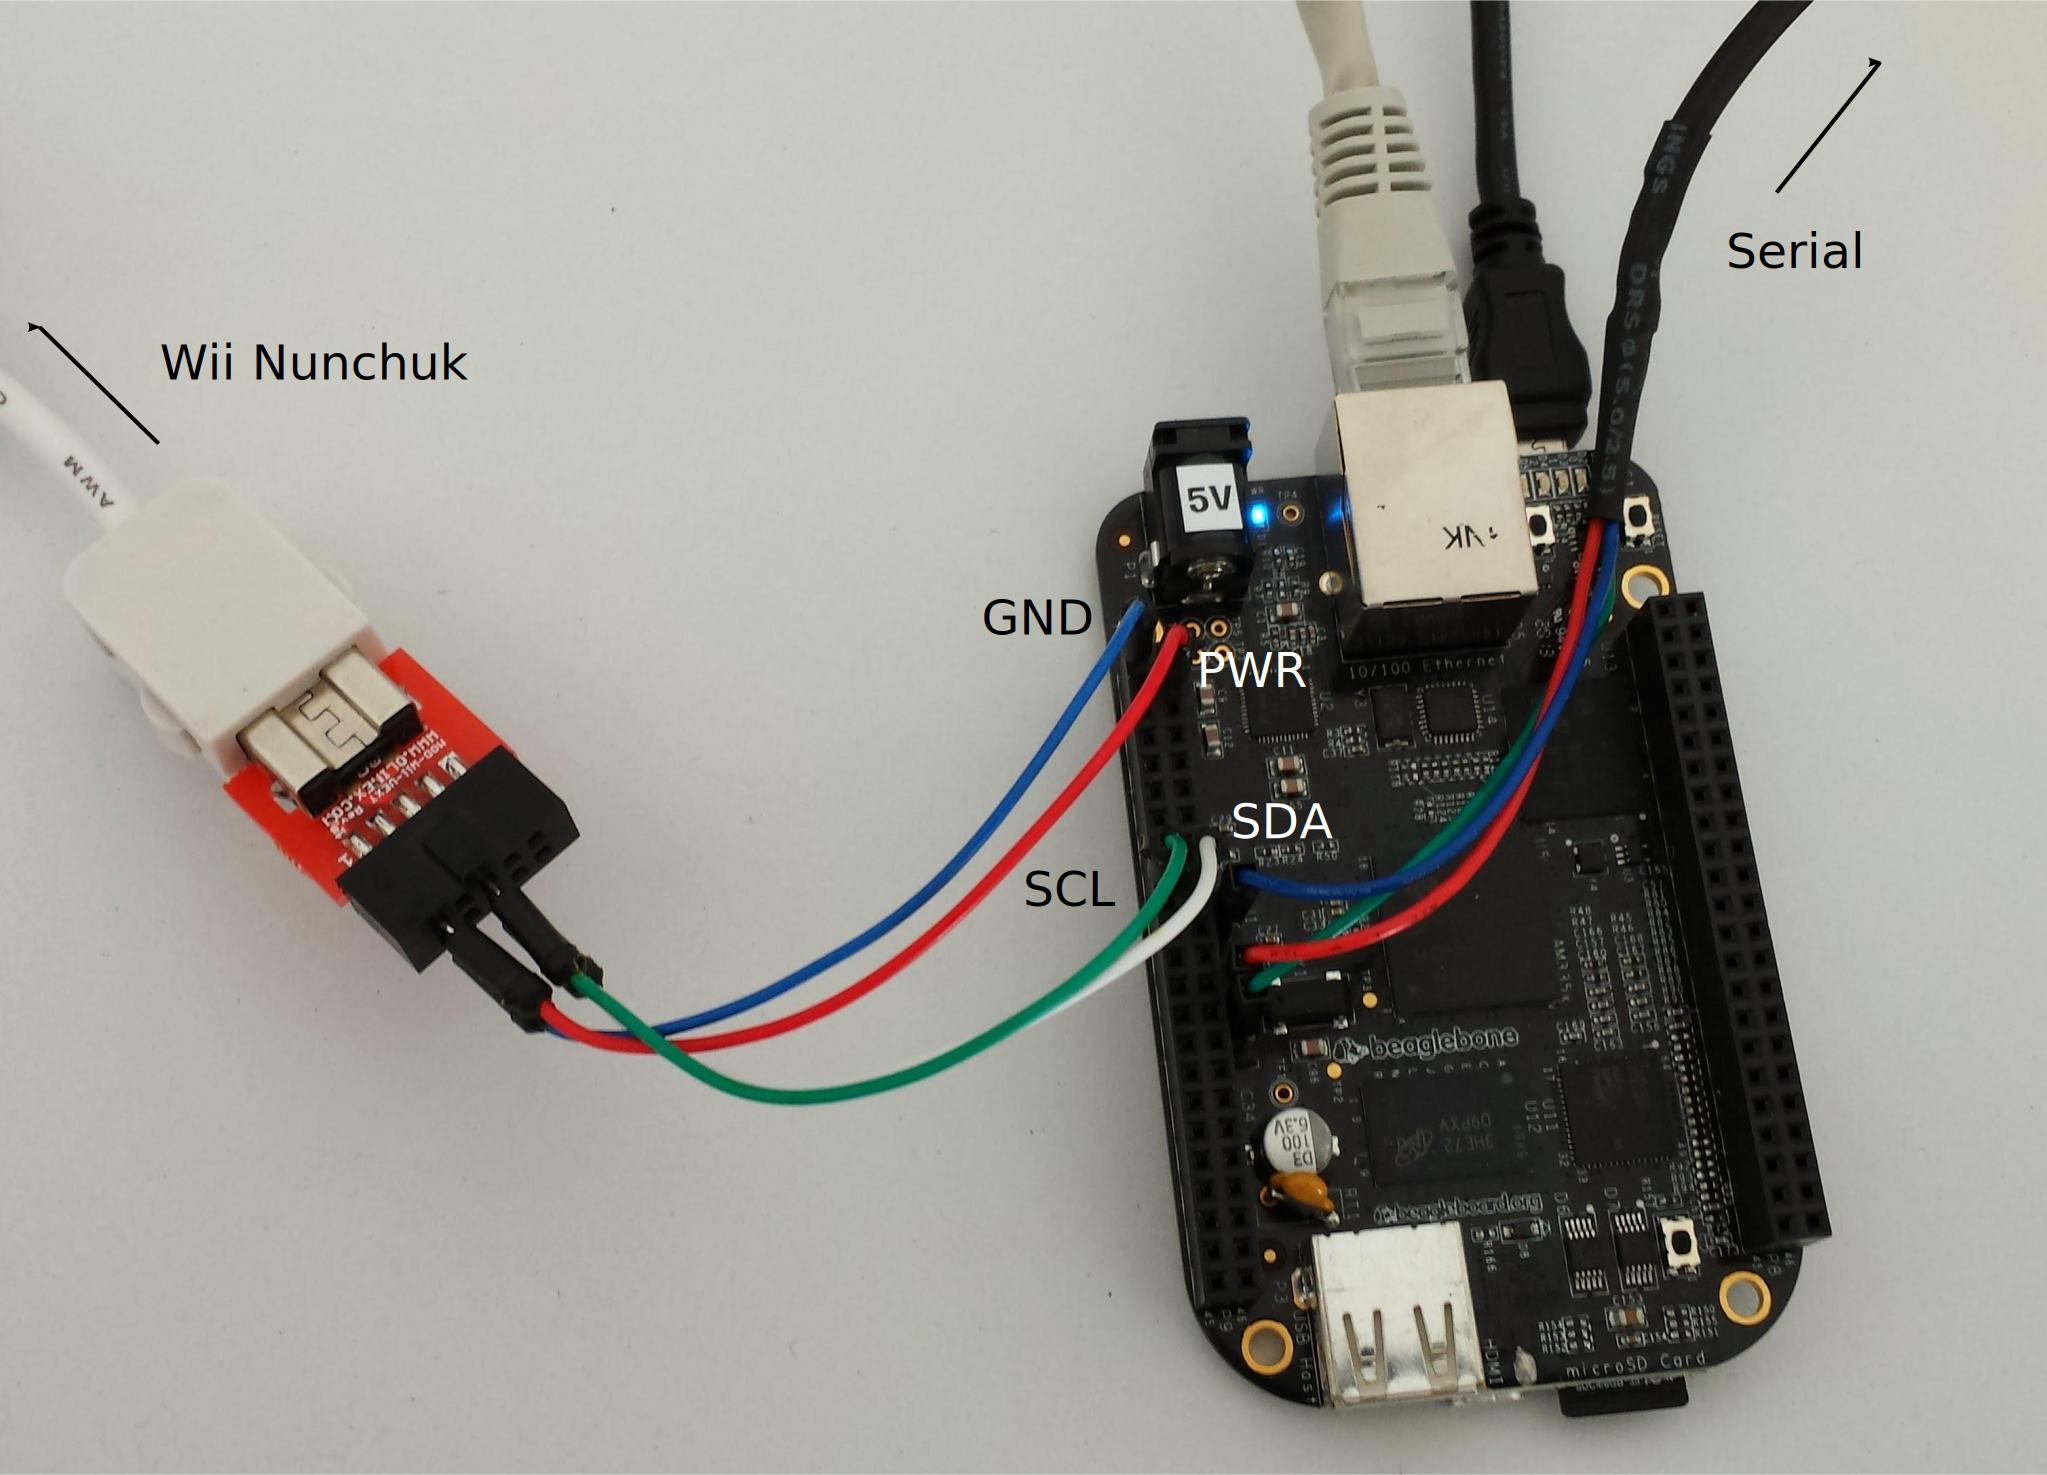
\includegraphics[width=12cm]{common/bbb-connect-nunchuk.pdf}
\end{center}
}

\section{Test the Nunchuk}

Copy the newly generated kernel and device tree images into the first SD card
partition. Then boot the board and wait until you have access to the
\code{busybox} command line.

You can then make sure that the Nunchuk is recognized and is working by
checking the presence of the \code{js0} device file:
\begin{verbatim}
ls /dev/input/js0
\end{verbatim}

Now display the raw events generated by the Nunchuk:
\begin{verbatim}
cat /dev/input/js0
\end{verbatim}

You should see random characters appearing while playing with the Nunchuk. Be
aware that the driver we integrated also handles accelerometer events. Therefore,
moving the device will produce many events!

\section{Patch nInvaders}

The nInvaders game uses keyboard events for its controls. We first need to apply
a patch introducing joystick support. The patch is located at
\code{~/yocto-labs/bootlin-lab-data/nunchuk/ninvaders/}.

Add the patch to the nInvaders \code{SRC_URI}.

Then build a full \code{core-image-minimal} and update the NFS root
directory.

\section{Play nInvaders!}

After booting the board you should be able to play nInvaders with the
keyboard\dots and the Nunchuk! The \code{C} button is used to confirm and to
fire, and \code{Z} to pause the game.

Access the board command line through SSH, and launch the game:
\begin{verbatim}
$ ninvaders
\end{verbatim}
